
\chapter{Scripting}
\label{ch:scripting}

\section{Introduction}
\label{sec:scripting:introduction}

Since version 0.10.1, Stellarium includes a scripting feature based on
the Qt Scripting
Engine\footnote{\url{http://doc.qt.io/qt-5/qtscript-index.html}}. This
makes it possible to write small programs within Stellarium to produce
automatic presentations, set up custom configurations, and to automate
repetitive tasks. 

The programming language
ECMAscript\footnote{\url{https://en.wikipedia.org/wiki/ECMAScript}}
(also known as JavaScript) gives users access to all basic ECMAScript
language features such as flow control, variables, string manipulation
and so on.

Interaction with Stellarium-specific features is done via a collection
of objects which represent components of Stellarium itself.  The
various modules of Stellarium, and also activated plugins, can be
called in scripts to calculate, move the scene, switch on and off
display of objects, etc.  You can write text output into text files
with the \command{output()} command.  You can call all public slots
which are documented in the scripting API documentation\footnote{\url{http://www.stellarium.org/doc/0.15.0/scripting.html}}.


\section{Script Console}
\label{sec:scripting:console}
It is possible to open, edit run and save scripts using the script
console window. To toggle the script console, press \key{F12}. The
script console also provides an output window in which script
debugging output is visible. 

\section{Includes}
\label{sec:scripting:includes}

Stellarium provides mechanism for splitting scripts into different
files. Typical functions or lists of variables can be stored in
separate \file{.inc} files and used within other scripts through the
\textbf{include()} command:
\begin{script}
include("common_objects.inc");
\end{script}


\section{Minimal Scripts}
\label{sec:scripting:MinimalScript}
This script prints ``Hello Universe'' in the Script Console log window and into \file{log.txt}. 
\begin{script}
core.debug("Hello Universe");
\end{script}

\noindent This script prints ``Hello Universe'' in the Script Console output window and \file{output.txt}. 
\begin{script}
core.output("Hello Universe");
\end{script}
The file \file{output.txt} will be rewritten on each run of Stellarium. In case you need to save a copy of the current output file to another file, call 
\begin{script}
core.saveOutputAs("myImportantData.txt");
core.resetOutput();
\end{script}

\noindent This script uses the LabelMgr module to display ``Hello Universe'' in red, fontsize 20, on the screen for 3 seconds.
\begin{script}
var label=LabelMgr.labelScreen("Hello Universe", 200, 200, 
                               true, 20, "#ff0000");
core.wait(3);
LabelMgr.deleteLabel(label);
\end{script}

\section{Retrograde motion of Mars}
\label{sec:scripting:RetrogradeMotionOfMars}
A best way begin writing of scripts --- to set for itself a specific goal and try to achieve it with the help of few simple steps. Any complex script can split on simple parts or tasks, which may solve any newbies in scripting. 

Let me explain it with examples.

Imagine that you have set a goal to make the demonstration is very beautiful, but long enough phenomenon --- the retrograde motion of the planet Mars (Fig.~\ref{fig:scripting:mars2005}). 

\begin{figure}[ht]
\centering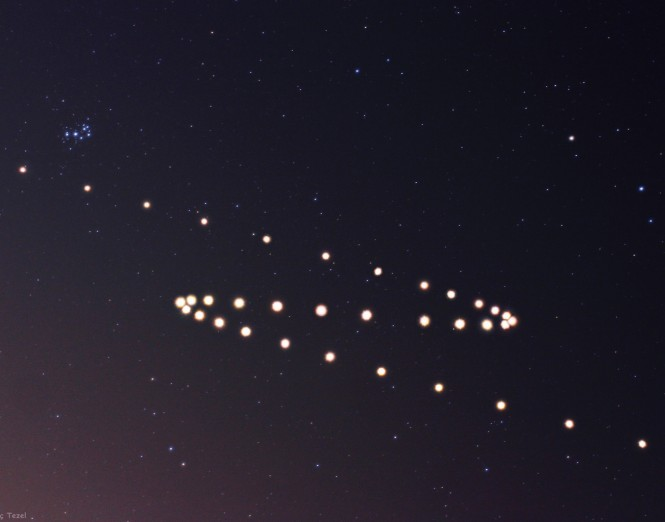
\includegraphics[width=300px]{Mars2005_tezel.jpg}
\label{fig:scripting:mars2005}
\caption{Retrograde motion of Mars in 2005. Credit \& Copyright: Tunc Tezel --- APOD: 2006 April 22 -- Z is for Mars.}
\end{figure}

\subsection{Script header...}
Any ``complex'' script contains a few lines in first part of file, which contains an important data for humans --- name of script and him description --- and some rules for Stellarium.

\begin{script}
//
// Name: Retrograde motion of Mars
// Author: Alexander Wolf
// License: Public Domain
// Version: 1.0
// Description: A demo of retrograde motion of Mars.
//
\end{script}
.....
\begin{script}
core.setJD(2453552.0); // July 1, 2005
\end{script}

\section{More Examples}
\label{sec:scripting:examples}
The best source of examples is the \file{scripts} sub-directory of the
main Stellarium source tree. This directory contains a sub-directory
called \file{tests} which are not installed with Stellarium, but are
nonetheless useful sources of example code for various scripting
features\footnote{The directory can be browsed online at
  \url{http://bazaar.launchpad.net/~stellarium/stellarium/trunk/files/head:/scripts/}. Script
  files end in \file{.ssc} and include files (which are not runnable
  by themselves) in \file{.inc}. Download links are to the right.}.



% TODO: More examples? 

%%% Local Variables: 
%%% mode: latex
%%% TeX-master: "guide"
%%% End: 
